\chapter{Implementation} \label{c:impl}

\section{Virtual Function I/O}
Virtual Function I/O (VFIO) is an IOMMU agnostic framework for exposing devices to userspace.

To use the IOMMU we need to initialize the IOMMU, VFIO, DMA and the NVMe device:
\begin{enumerate}
    \item \textbf{Initialize the IOMMU: } First, we need to initialize the IOMMU. This is done using the VFIO IOMMU API, which is an interface for the IOMMU driver. % todo
    \item \textbf{Initialize the VFIO group: }
    \item \textbf{Enable DMA in the PCI configuration space of the NVMe device}
    \item \textbf{Use \texttt{mmap} to map NVMe base address register to memory}
\end{enumerate}

VFIO consists of two parts, the \texttt{vfio-pci} driver and an IOMMU API (\texttt{vfio\_iommu\_type1}). The VFIO PCI driver can be bound to a PCI device. This allows using \texttt{mmap(2)} to map the PCI device registers into memory. The type1 VFIO IOMMU API is used for mapping and unmapping address translations in the IOMMU. Alternatively, the IOMMUFD API can be used instead of the container API, which currently is not feature complete, but will eventually replace the container based solution \cite{vfiokerneldocs}.
This allows the driver to be safe and non-privileged in comparison to directly mapping the device memory to userspace.
Using the VFIO works by using ioctl system calls.
While there is Rust's extensive \texttt{libc} library providing the system calls \texttt{ioctl} and \texttt{mmap} and their flags, the Linux \texttt{vfio.h} constants and structs need to either be defined manually or with a crate like bindgen, which automates bindings for C and C++ libraries \cite{cratebindgen}. To keep the binary and dependency list as small as possible we chose the manual implementation.

Using \texttt{VFIO\_IOMMU\_GET\_INFO} we can see the supported pagesizes. As our IOMMU supports 4K, 2M and 1G pagesizes the field iova\_pgsizes has the value 0x40201000.

\section{syscalls}
A variety of syscalls are used in the process of allocation and mapping. These syscalls are mmap, ioctl, pread, pwrite (and mlock for the non IOMMU version). While there exist crates which implement the syscall functionality, to avoid inflating the dependency list and executable size we use the libc crate to implement them. As these require C-like syntax and an unsafe block in Rust, wrapper macros are used to provide locality of behaviour, secure error handling, while also minimising the calling of unsafe code. In \autoref{lst:mmapmacro} the macro for the mmap syscall can be seen.
As part of our error handling, we introduce an error enum variant for each syscall. The macro is marked as unsafe in its name in order to not hide any unsafe code.

\begin{lstlisting}[language=Rust,caption={Syscall \texttt{mmap} macro, with own error variant}, label=lst:mmapmacro]
    #[macro_export]
    macro_rules! mmap_unsafe {
        ($addr:expr, $len:expr, $prot:expr, $flags:expr, $fd:expr, $offset:expr) => {{
            let ptr = unsafe { libc::mmap($addr, $len, $prot, $flags, $fd, $offset) };
            if ptr == libc::MAP_FAILED {
                Err(Error::Mmap {
                    error: (format!("Mmap with len {} failed", $len)),
                    io_error: (std::io::Error::last_os_error()),
                })
            } else {
                Ok(ptr)
            }
        }};
    } 
\end{lstlisting}

\subsection{Binding NVMe to \texttt{vfio-pci}}

To use the IOMMU for the driver, we first need to initialize the VFIO kernel module and bind the VFIO driver to the NVMe device.
As this binds the driver to a device, it has to be run with root privileges.
By changing the owner of the VFIO container to an unprivileged user, the driver can use the VFIO driver to interact with the device without root.
In \autoref{lst:vfioinit} the initialization script for the Vfio driver is shown.

% maybe take vfio_bind function
\begin{lstlisting}[language=bash,caption={Initializing VFIO using bash}, label=lst:vfioinit, frame=single]
    #!/bin/bash
    modprobe vfio-pci
    nvme_vd="$(cat /sys/bus/pci/devices/$nvme/vendor) $(cat /sys/bus/pci/devices/$nvme/device)"
    echo $nvme > /sys/bus/pci/devices/$nvme/driver/unbind
    echo $nvme_vd > /sys/bus/pci/drivers/vfio-pci/new_id
    chown $user:$group /dev/vfio/*     
\end{lstlisting}

\begin{enumerate}
    \item Add VFIO kernel module using \texttt{modprobe}
    \item Unbind kernel driver from NVMe
    \item Use vendor and device id to bind VFIO to the device
    \item Set VFIO group permissions to user/group using \texttt{chown}
\end{enumerate}

\subsection{Initialising the IOMMU}
To initialise the IOMMU, we first need to get the container file descriptor. The container is accessible under the path \texttt{/dev/vfio/vfio}. Using the raw container file descriptor, we can use the following \texttt{ioctl} calls to initialise the IOMMU.

\begin{lstlisting}[language=Rust, caption={ioctl calls needed for IOMMU initialization}, label=lst:containerioctls]
    ioctl_unsafe!(container_fd, VFIO_GET_API_VERSION)
    ioctl_unsafe!(container_fd, VFIO_CHECK_EXTENSION, VFIO_TYPE1_IOMMU)
    ioctl_unsafe!(group_fd, VFIO_GROUP_GET_STATUS, &group_status)
    ioctl_unsafe!(group_fd, VFIO_GROUP_SET_CONTAINER, &container_fd)
    ioctl_unsafe!(container_fd, VFIO_SET_IOMMU, VFIO_TYPE1_IOMMU)
    ioctl_unsafe!(group_fd, VFIO_GROUP_GET_DEVICE_FD, pci_addr)
    ioctl_unsafe!(container_fd, VFIO_IOMMU_GET_INFO, &iommu_info)   
\end{lstlisting}

Excluding the Status and Info calls, the functionality consists of initialising the IOMMU for the device groups by setting the container on the groups, enabling Type1 for the IOMMU and fetching the device file descriptor. With the device file descriptor, we gain access to the device regions through the VFIO device API, allowing us to \texttt{mmap} the NVMe BAR into memory.

\subsection{Initialising the NVMe device}
Using the Vfio, the initialization process of the NVMe SSD works as followed.

\begin{enumerate}
    \item Map the NVMe device memory into host memory using VFIO resource info.
    \item Allocate Admin SQ, CQ and I/O SQ, CQ
    \item Create a mapping on the IOMMU using VFIO
    \item Configure the NVMe device
    \item Pass I/O Queue addresses to NVMe device using admin queues
\end{enumerate}

\subsection{DMA}
To enable DMA we need to set a bit in the PCIe device registers. % todo check this 
This is done in the command register of the PCIe configuration space.

\paragraph{Mapping DMA}
In order to provide a section of memory on which the device can perform DMA operations, the user needs to allocate some memory in the processes address space. This can be achieved by using the Linux syscall \texttt{mmap}. Using \texttt{mmap}'s flags we can also define the page size used. The \texttt{MAP\_HUGETLB} flag is used in conjunction with the \texttt{MAP\_HUGE\_2MB} and \texttt{MAP\_HUGE\_1GB} flags for 2MiB and 1 GiB pages respectively. By default \texttt{mmap} uses the default page size of 4KiB.
The main IOMMU work is done by then creating the map struct \texttt{vfio\_iommu\_type1\_dma\_map}. We set the DMA mapping to read and write, and provide the same IOVA as the Virtual address. By then passing it to an ioctl call with the according VFIO operation \texttt{VFIO\_IOMMU\_MAP\_DMA} we can create a mapping in the page tables of the IOMMU. This way we can give the IOVA to the NVMe controller, which it will use to access the memory through the address translation of the IOMMU.

\begin{lstlisting}[language=Rust,caption={Mapping memory for DMA}, label=lst:mapdma]
    let mut iommu_dma_map = vfio_iommu_type1_dma_map {
        argsz: mem::size_of::<vfio_iommu_type1_dma_map>() as u32,
        flags: IoctlFlag::VFIO_DMA_MAP_FLAG_READ 
                | IoctlFlag::VFIO_DMA_MAP_FLAG_WRITE,
        vaddr: ptr as u64,
        iova: ptr as u64,
        size,
    };

    ioctl_unsafe!(
        *container_fd,
        IoctlOperation::VFIO_IOMMU_MAP_DMA,
        &mut iommu_dma_map
    )?;

    let iova = iommu_dma_map.iova as usize; 
\end{lstlisting}

\newpage

\begin{figure}
    \centering
    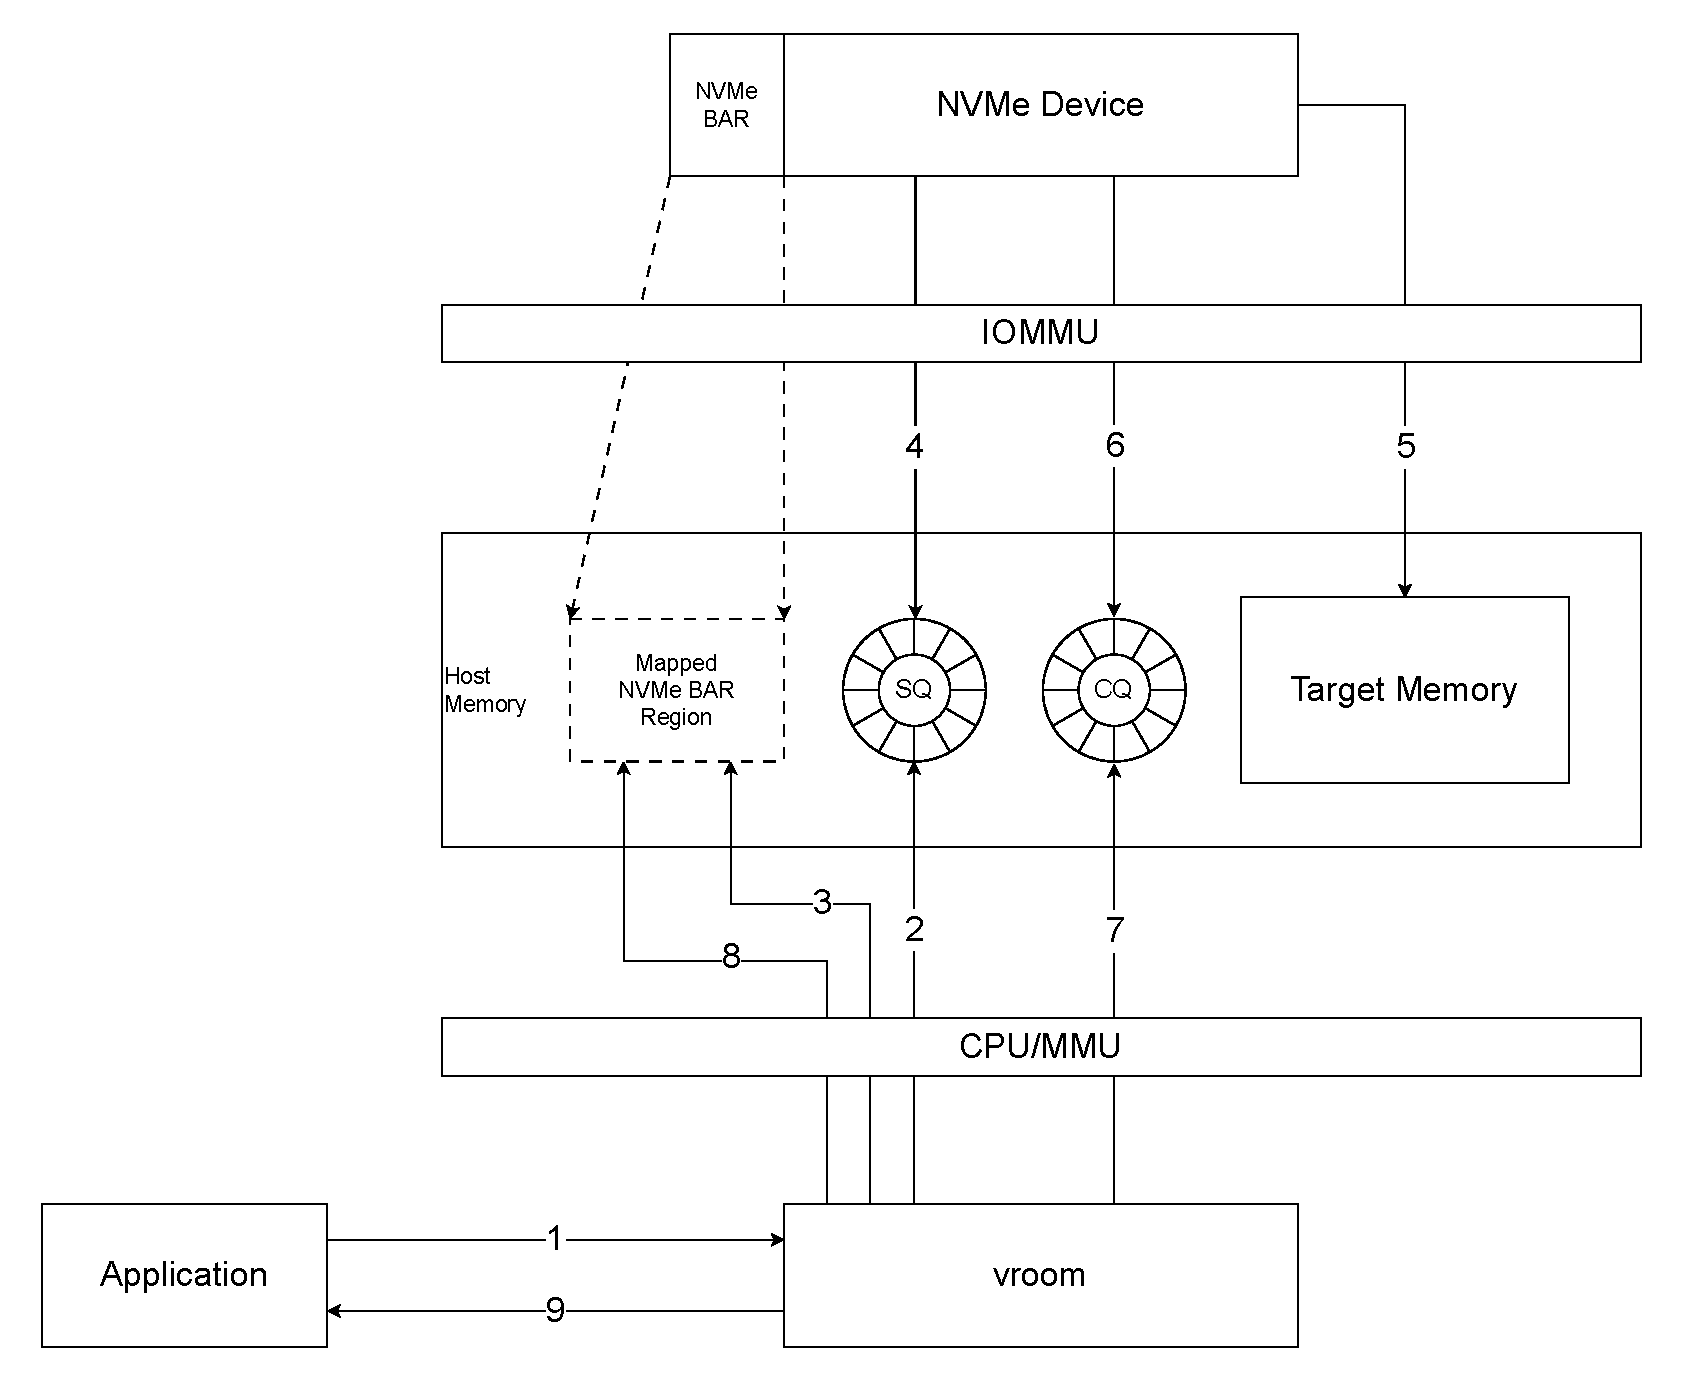
\includegraphics[width=\textwidth]{figures/vroomdiagram.pdf}
    \caption{I/O operation using vroom with enabled IOMMU}
    \label{fig:vroom-graph}
\end{figure}
On \autoref{fig:vroom-graph} an I/O operation timeline graph can be seen. The timeline is described as followed:
\begin{enumerate}
    \item \textbf{I/O function call:} The application calls a read/write method on vroom
    \item \textbf{Command Submission:} Vroom creates a \texttt{NvmeCommand} struct and places it on the Submission Queue head.
    \item \textbf{Ring SQ Doorbell:} Vroom places the submission queue head address in the doorbell register. The doorbell register is part of the NVMe BAR region, which is mapped to memory.
    \item \textbf{Take Command:} The NVMe takes the command from the SQ.
    \item \textbf{Perform I/O:} The NVMe uses the IOMMU to access the host memory via DMA and performs the read/write command.
    \item \textbf{Complete I/O:} The NVMe places a \texttt{NvmeCompletion} struct instance on the head of the Completion Queue.
    \item \textbf{Polled CQ:} By polling the CQ, vroom can process the CQ entry.
    \item \textbf{Ring CQ Doorbell:} After processing the CQ entry, vroom rings the CQ Doorbell, in order to notify the NVMe controller, that the Completion Queue has been processed.
    \item \textbf{Notify Application:} Vroom notifies the Application of the success of the I/O operation. The application can continue running.
\end{enumerate}



\paragraph{Unmapping DMA}
Unmapping DMA happens when the process exits, yet for performance and application reasons we implement the unmap\_dma function which can be used to unmap a DMA. Using the \texttt{VFIO\_IOMMU\_UNMAP\_DMA} \texttt{ioctl} operation we can unmap the memory, and finally free it by using \texttt{munmap}.

\subsection{Regions}
Using regions, we can directly mmap device memory into host memory for easy access to the NVMe controller.
VFIO provides structs for using mmap to directly map the NVMe device into memory. Using \texttt{VFIO\_DEVICE\_GET\_REGION\_INFO} we can attain the length and the offset needed for mmap.

\subsection{Groups and Containers}
VFIO uses group to distinguish between groups of devices which can be isolated from the host system. In the ideal case, every device would only be part of one group in order to increase security by providing single-device isolation. Groups are the smallest unit size on a system to ensure secure user access.
To further reduce overhead from the IOMMU Containers are used in VFIO, which can hold multiple groups. These containers can be used to ease translation and reduce TLB page faults.
% In our implementation we use one group and container each for our NVMe device.

\section{IOMMUFD}
The IOMMU File Descriptor user API (IOMMUFD) offers a way of controlling the IOMMU subsystem using file descriptors in user-space \cite{iommufdkerneldocs}. It replaces the VFIO IOMMU API using containers with the IOMMUFD API.
It allows management of I/O address spaces (IOAS), enabling mapping user space memory on the IOMMU.
IOMMUFD has only been recently added to the Linux Kernel in December 2022. E.g. Debian 12 does not include it, Fedora 40 does, but it is not enabled in the kernel configuration. Considering that it is not widely available or enabled on many distributions, our driver offers both options of using the IOMMU. The performance tests are done using the 'legacy' VFIO container way.
The device file descriptor, which was previously attained with \texttt{VFIO\_GROUP\_GET\_DEVICE\_FD} can now be gotten through opening the character device /dev/vfio/devices/vfioX.
By using this character device pointer we can claim the ownership over the VFIO device. That way VFIO does not rely on group/container/iommu drivers.
I/O Address Spaces (IOAS) are the equivalent to a VFIO container in legacy VFIO.

\begin{figure}
    \centering
    \subcaptionbox {VFIO with Containers} {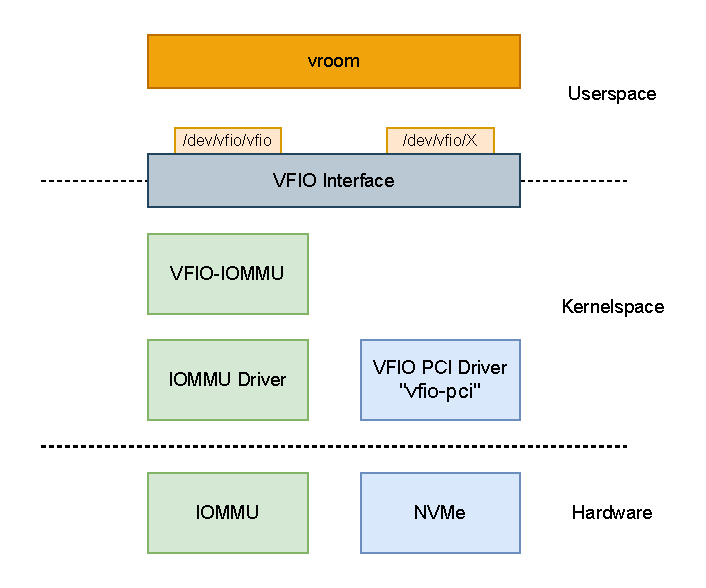
\includegraphics[width=0.67\textwidth]{figures/VFIOLayer.pdf} \label{fig:layer-vfio}}
    \subcaptionbox {VFIO with IOMMUFD (IOAS)} {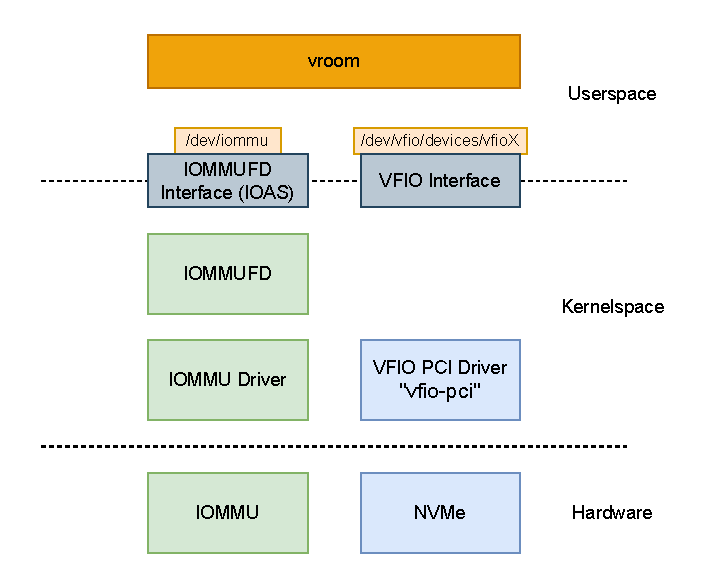
\includegraphics[width=0.67\textwidth]{figures/IOMMUFDLayer.pdf} \label{fig:layer-iommufd}}
    \caption{Layer diagrams of VFIO with VFIO Container API and IOMMUFD, partly adopted from \cite{dpdkiommufd}}
    \label{fig:clayer}
\end{figure}
